\chapter{مقدمه}\label{Chap:Chap1}
\minitoc
در این فصل ابتدا به معرفی مساله‌ی تولید دنباله می‌پردازیم، اهمیت و کاربرد‌های این مساله را مورد بررسی قرار می‌دهیم. پس از آن به صورت مختصر درباره‌ی یادگیری 
\trans{مقابله‌ای}{Adversarial}
و دلیل توجه به آن توضیحاتی می‌دهیم. سپس چالش‌هایی ذاتی مساله، چالش‌هایی که در روش‌های پایه برای حل مساله وجود داشته و چالش‌های ایجاد شده با استفاده از یادگیری مقابله‌ای بیان می‌شود و فصل حاضر را با تشریح ساختار پایان‌نامه و فصول مختلف آن به پایان می‌بریم.
\section{تعریف مساله}
\label{sec:chap1:definition}
در این پژوهش هدف تولید دنباله‌های گسسته با آموزش بر روی نمونه‌هایی که از این دنباله داریم است.
دنباله‌ی گسسته به معنی تعدادی متغیر گسته است که ترتیب دارند و گسسته بودن دنباله به این معنی است که هر مقدار دنباله مقادیر محدودی می‌گیرد. در این پژوهش داده‌ی گسسته از نوع 
\trans{دسته‌ای}{Categorical}
مدنظر است (در مقابل داده‌های عددی مثل مجموعه‌ی اعداد صحیح). در داده‌های دسته‌ای همه‌ی مقادیر ممکن هم‌فاصله است، از این رو معمولا این مقادیر به صورت بردار
\trans{یک-فعال}{One-hot}
کد می‌شوند. هر یک از این مقادیر در دنباله را کلمه می‌نامیم.
\newpage
برای مثال یک نمونه از دنباله‌ی گسسته به صورت زیر است:
\begin{equation*}
\underbrace{\clubsuit}_{\text{عنصر اول}}
 \diamondsuit \bigstar \clubsuit \clubsuit \heartsuit \spadesuit \heartsuit \bigstar \clubsuit \clubsuit \spadesuit \heartsuit \heartsuit,
\end{equation*}

که از چپ به راست ترتیب دارند، هر یک از عناصر یکی از مقادیر 
$\{ \clubsuit , \diamondsuit ,\bigstar , \spadesuit , \heartsuit \} $
را به خود گرفته است و میزان شباهت هر دو مقداری از این مجموعه با همدیگر مساوی است.
\section{اهمیت و کاربرد}
داده‌های زیادی را می‌توان با دنباله مدل کرد، از این رو موضوع تولید دنباله دامنه‌ی وسیعی را در بر می‌گیرد.
در ادامه با ذکر تعدادی از این حوزه‌ها برای آن کاربرد‌هایی ذکر می‌شود و اهمیت آن تشریح می‌شود.
\begin{itemize}
	\item 
	\textbf{ زبان طبیعی:}
زبان طبیعی را می‌توان	دنباله‌ای از کلمات و یا حروف درنظر گرفت، تولید زبان طبیعی در ترجمه‌ی متن، سیستم‌های پاسخگویی خودکار، خلاصه‌سازی متن، تولید عنوان برای تصاویر و غیره کاربرد دارد.
هر یک از این مثال‌ها خود حوزه‌ی پراهمیتی است که به صورت جداگانه مورد پژوهش هستند.
بهبود مساله‌ی تولید دنباله می‌تواند منجر به بهبود در کاربرد‌های ذکر شده شود. 
		\item 
		\textbf{ ساختار مولکولی:}
		ساختارهای مولکولی را می‌توان با رشته‌های به نام
		\lr{SMILES}
		بیان کرد
		\cite{weininger1988smiles}.
		این نحوه‌ی بیان اطلاعات هندسی ساختار مولکولی را در خود دارد. این رشته‌ها دارای قواعد گرامری هستند و لزوما هر رشته‌ای متناظر یک ساختار مولکولی نیست
		\cite{ORGAN}،
		از این رو نیاز به روش‌هایی احساس می‌شود که دنباله‌های معتبر با ویژگی‌های خواسته شده تولید کند. 
برای مثال اگر مدل برای یک داروی موردنظر ساختار‌های مولکولی ارائه دهد که ویژگی‌های خاصی را داشته باشند، فرایند تولید دارو‌های جدید و شخصی‌سازی شده ساده‌تر و اقتصادی‌تر می‌شود. مولکول‌ها فقط محدود به دارو نیستند و در حوزه‌ای مثل کشف مواد جدید هم این بحث‌ وجود دارد
		\cite{ORGAN}.
		\item 
		\textbf{ گراف :}
		به تازگی روش‌هایی بر مبنای
\trans{گشت‌زنی تصادفی}{Random Walk}
در حوزه‌ی گراف ارائه شده است که نتایج موفقی داشته‌اند.
 در این روش بجای کار روی ساختار گراف بر روی دنباله‌های حاصل از گشت‌زنی تصادفی روی گراف کار می‌شود. 
برای تولید گراف، دنباله‌هایی به عنوان گشت‌زنی تصادفی آن تولید می‌شود و از روی این دنباله‌ها گراف ساخته می‌شود.
موضوع تولید گراف شامل حوزه‌های کاربرد‌های زیادی می‌شود، برای مثال در تولید
\trans{گراف دانش}{Knowledge Graph}
و یا گراف ساختار مولکولی کاربرد دارد
		\cite{Aleksandar18NetGAN, Jiaxuan18GraphRNN}.
		
		\item 
		\textbf{ موسیقی:}
				یکی از راه‌های ذخیره‌سازی باکیفیت موسیقی ثبت نُت‌های آن است، از آنجا که این نت‌ها تعداد حالات محدودی دارند و در زمان ترتیب دارند می‌توان آن را به عنوان‌ دنباله‌هایی در طول زمان مدل کرد
				\cite{SeqGAN}.
\end{itemize}


\section{يادگیری مقابله‌ای}
\label{Method:GAN:Shalow}
\trans{شبکه‌های مولد مقابله‌ای}{Generative Adversarial Networks}
\cite{Goodfellow2014}
روشی برای آموزش مدل 
\trans{مولد}{Generative}
 است بر این مبنا که شبکه‌هایی با هم رقابت می‌کنند و به نوعی با هم بازی انجام می‌دهند؛ نتیجه‌ی این رقابت آموزش مدل مولد است.
روش‌های آموزش مبتنی بر این ایده را یادگیری مقابله‌ای می‌نامیم.
در ادامه به نحوه‌ی کار روش شبکه‌های مولد مقابله‌ای معرفی شده در
\cite{Goodfellow2014}
می‌پردازیم و سپس چند دلیل برای اهمیت یادگیری مقابله‌ای‌ ذکر می‌کنیم.
\newline
در شبکه‌های مولد مقابله‌ای برای آموزش مدل مولد از شبکه‌ی دومی به عنوان
\trans{تمیزدهنده}{Discriminator}
استفاده می‌شود، این شبکه‌ یک
\trans{دسته‌بند}{Classifier}
دو دسته‌ای است. روال آموزش به این صورت است که تمیزدهنده بین دو مجموعه داده‌ی واقعی و داده‌های تولید شده توسط مولد دسته‌بندی انجام می‌دهد، سپس شبکه‌ی مولد به سمتی سوق داده می‌شود که تمیزدهنده را به اشتباه بیاندازد و این دو مرحله به صورت تکراری انجام می‌شود.
 در این روش آموزش تمیزدهنده مشابه یک دسته‌بند عادی انجام می‌شود.
 از آنجا که شبکه‌ی تمیزدهنده نسبت به ورودی مشتق‌پذیر است برای آموزش مدل مولد، گرادیان از شبکه‌ی تمیزدهنده وارد شده و پارامتر‌های مدل مولد را به‌روزرسانی می‌کند، به عبارت دیگر شبکه‌ی تمیزدهنده مشابه تابع هزینه برای مولد عمل کرده و مشخص می‌کند با تغییر پارامتر‌های مولد در چه راستایی تمیزدهنده به اشتباه می‌افتد.
\subsection{دلیل توجه به یادگیری مولدمقابله‌ای}
برای حل مساله‌ی تولید دنباله توجه زیادی به آموزش مقابله‌ای شده است
\cite{kusner2016gans,lamb2016professor,Zhang2017TextGAN,SeqGAN,ORGAN,lin2017adversarial,Guo2018,Che2017,press2017langwasserstein}،
در ادامه دلایلی برای این موضوع ذکر می‌کنیم.
	\begin{figure}[!htb]
		{
			\begin{center}
				\subfigure[تصاویر مصنوعی تولید شده]{\label{Figure:NVIDIAGAN:Sample}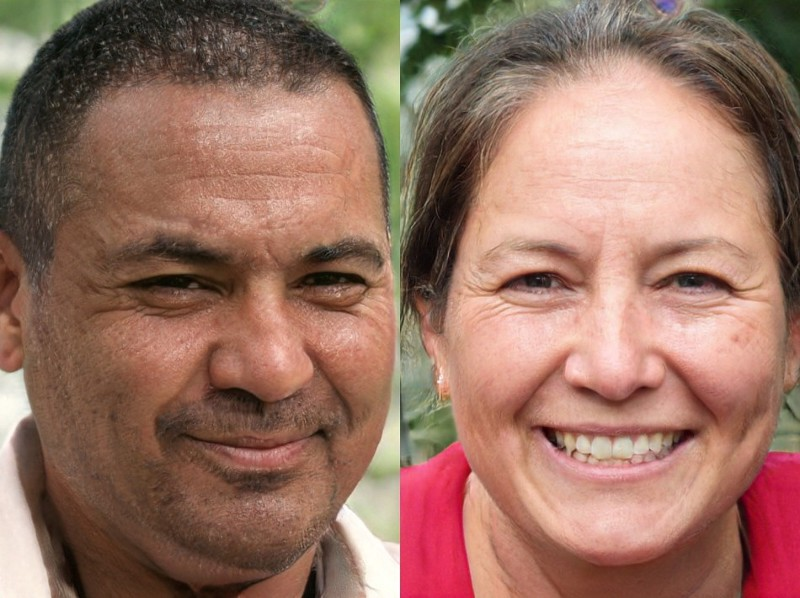
\includegraphics[scale=0.25]{images/Nvidia/SelectedGenerated.png}}
				\hspace{1cm}
				\subfigure[
				ادغام تصاویر در فضای ویژگی و تبدیل تصاویر مبدا به سبک تصویر مقصد
				]{\label{Figure:NvidiaGAN:Latent}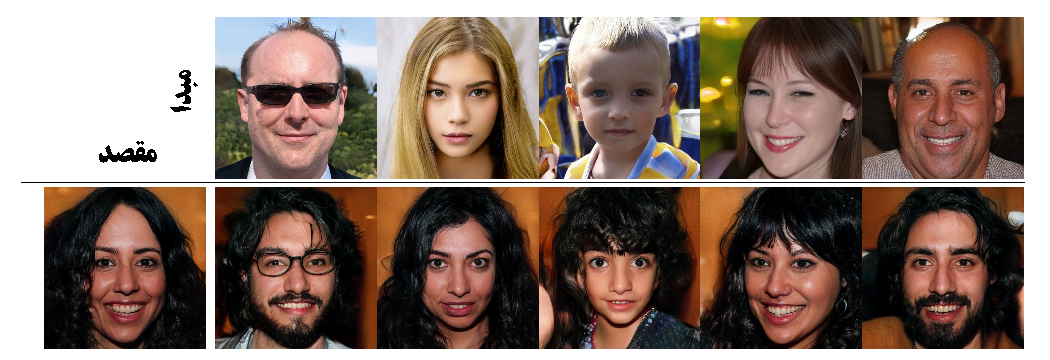
\includegraphics[scale=0.8]{images/Nvidia/SelectedStyle2.pdf}} 
				\end{center}
			\caption[نتایج یکی از آخرین پژوهش‌های انجام شده در حوزه‌ی تصویر با کمک شبکه‌های مولد مقابله‌ای]{
				نتایج یکی از آخرین پژوهش‌های انجام شده در حوزه‌ی تصویر با کمک شبکه‌های مولد مقابله‌ای
				\cite{karras2018style}
			}
			\label{Figure:NVIDIAGAN:SampleAndLatent}
		}
		\end{figure}

\begin{itemize}
	\item 
	\textbf{پیشرفت‌های چشم‌گیر یادگیری مقابله‌ای در حوزه‌ی تصویر:}
	بعد از معرفی یادگیری مقابله‌ای، این روش در حوزه‌ی تولید تصویر نتایج
	\trans{مرز دانش}{State-of-the-Art}
	را کسب کرده است و هر روزه شاهد پیشرفت‌های بیشتری در این حوزه با کمک یادگیری مقابله‌ای هستیم.
	\newline
	برای مثال در یکی از جدیدترین پژوهش‌هایی که توسط یک شرکت بزرگ ساخت کارت‌های گرافیکی بر روی تولید تصویر صورت انسان انجام شده است
	\cite{karras2018style}،
نتیجه‌ی این پژوهش علاوه بر کسب امتیاز بالایی در معیار ارزیابی مربوط به آن حوزه، موفق به تولید تصاویر بسیار نزدیک به تصاویر واقعی شده است.
به طوری که نمونه‌های ارائه شده در مقاله بسیار باکیفیت هستند و مصنوعی بودن آن غیرقابل تشخیص است، در شکل 
	\ref{Figure:NVIDIAGAN:Sample}
	دو نمونه از این تصاویر نمایش داده شده است. به علاوه فضای
	\trans{نهان}{Latent}
	که بر روی تصاویر صورت به دست آمده با معنی بوده و قابلیت ترکیب تصاویر تولید شده را می‌دهد، برای مثال شکل
	\ref{Figure:NvidiaGAN:Latent}
	نشان دهنده‌ی چند تصویر ورودی در سطر اول است که با کمک فضای ویژگی به دست آمده، به
	\trans{سبک}{Style}
	تصویر سمت چپ تبدیل شده‌اند. به این ترتیب، به واسطه‌ی عملکرد مناسب این روش‌ها در حوزه‌ی تولید تصویر، در دو سال اخیر توجه به سمت استفاده از مدل‌های مولدمقابله‌ای در حوزه‌ی تولید متن هم جلب شده است.
	\item 
	\textbf{قابلیت استفاده از دسته‌ی بزرگی از فاصله‌ها: }
	اثبات شده است که آموزش به وسیله‌ی شبکه‌های مولد مقابله‌ای،
 معادل کاهش فاصله‌ی
\lr{Jensen-Shannon}
بین توزیع اصلی و توزیع مولد است
\cite{Goodfellow2014}.
هم‌چنین روش‌های مبتنی بر یادگیری مقابله‌ای برای کاهش فاصله‌های دیگر هم پیشنهاد شده است
\cite{Nowozin2016, Poole2016}.
این فاصله‌ها روش مستقیم برای استفاده به عنوان
\trans{تابع هزینه‌}{Cost Function}
  ندارند و این امر با کمک یادگیری مقابله‌ای محقق شده است.
	\item 
	\textbf{کمک به حل بعضی مشکلات موجود در روش‌های پایه:}
	در روش‌های پایه‌ی تولید دنباله مشکلاتی مثل
 \trans{اُریبی مواجهه}{Exposure Bias}
	وجود دارد که دلیل آن رفتار متفاوت مولد در دو فاز 
\trans{آموزش}{Train}
	 و 
\trans{آزمون}{Test}
	 است. در ادامه در بخش چالش‌ها بیشتر به این موضوع می‌پردازیم.
 معمولا روش یادگیری مقابله‌ای دچار این مشکل نمی‌شوند، زیرا اکثر این روش‌ها فاز آموزش و آزمون یکسانی برای تولید دنباله دارند.
\end{itemize}

\section{چالش‌ها}\label{ch1:dooshvari}
در این بخش ابتدا به چالش معیار ارزیابی و تابع هزینه که چالش ذاتی مساله است می‌پردازیم، در ادامه نمونه‌ای از مشکل روش پایه را بیان کرده و در پایان مشکلات استفاده از یادگیری مقابله‌ای را در مساله بیان می‌کنیم.
\subsection{مشخص نبودن معیار ارزیابی مناسب}
در حوزه‌ی مدل‌های مولد معیار ارزیابی مشخصی وجود ندارد و نحوه‌ی ارزیابی این مدل‌ها خود یک چالش است
\cite{Lucas15NoteOnEvaluation}.
ارزیابی مدل‌های مولد دنباله هم از این قاعده مستثنی نیست و معیاری استانداردی به جز قضاوت انسانی وجود ندارد. به دلیل اهمیت معیار ارزیابی، فصل
\ref{Chap:Chap4}
به این موضوع اختصاص داده‌شده است.
\subsection{مشخص نبودن تابع هزینه مناسب}
مشکلی مشابه در حوزه‌ی انتخاب تابع هزینه مورد استفاده وجود دارد و بخش عمده‌ای از پژوهش‌های انجام شده در حوزه‌ی تولید دنباله به روش‌های آموزش و تابع‌های هزینه اختصاص دارد.
\newline
\trans{تابع هدف}{Objective Function}
اولیه مورد استفاده در روش‌های پایه مبتنی بر  
\trans{بیشینه درست‌نمایی}{Maximum Likelihood}
است. این تابع هدف به این معنی است که در آموزش مدل، هدف افزایش احتمالی است که مدل به داده‌های آموزش می‌دهد و به سمتی می‌رود که از دید مدل، داده‌های واقعی احتمال بالایی بگیرند؛
ولی اینکه به دنبال مدل‌هایی باشیم که نمونه‌های تولیدی آن در توزیع واقعی داده‌ها (که در دسترس نیست) احتمال بالایی بگیرند، رویکرد منطقی‌تری است. با این وجود راه‌حلی برای استفاده از این تابع هدف وجود ندارد.
روش‌های یادگیری مقابله می‌توانند استفاده از تابع هدف‌های بهتر را ممکن کنند
\cite{Huszar15HowNot}.
درست‌نمایی مدل را به سمتی می‌برد که به داده‌های آموزش احتمال بالایی دهد، ولی این موضوع را کمتر در نظر می‌گیرد که به نمونه‌های غیر از داده‌های آموزش احتمال کمی نسبت دهد. این ویژگی می‌تواند منجر به رفتاری شود که به نمونه‌ی نامعتبری احتمال بالا نسبت داده شود، این رفتار به نام 
 \trans{میانگین-جستجوگری}{Mean-Seeking}
شناخته می‌شود که در
ادامه بیشتر توضیح داده شده است.
 \subsubsection{رفتار میانگین-جستجوگری}
 در حالتی که ظرفیت مدل به اندازه‌ی کافی است با در نظر گرفتن تابع درست‌نمایی به عنوان تابع هدف می‌توان توزیع داده‌ی اصلی را یاد گرفت. 
 ولی در حالتی که ظرفیت مدل در مقابل داده‌های آموزش کم است مدل نمی‌تواند توزیع اصلی را کاملا یاد بگیرد و بسته به تابع‌ هزینه رفتار‌های متفاوتی را بروز می‌دهد. رفتاری که با تابع هدف درست نمایی بروز داده می‌شود باعث می‌شود توزیع آموزش دیده کل توزیع داده اصلی را در بر بگیرد و در این بین ممکن است به نقاطی از فضا بیشترین احتمال را نسبت دهد که دادها‌ی اصلی در آنجا احتمال کمی دارند. 
 این رفتار میانگین-جستجوگری نامیده می‌شود.
 در حوزه‌ی مدل‌های مولد این رفتار به این معنی است که مدل می‌خواهد داده‌هایی شبیه به تمام داده‌های آموزش تولید کند، حتی به این قیمت که بعضی از داده‌های تولیدی شبیه به داده‌های آموزش نباشد
 \cite{Huszar15HowNot}.
 به صورت کلی‌تر رفتار میانگین-جستجوگری مربوط به استفاده فاصله‌ی 
\lr{Kullback-Leibler (KL)}
 بین توزیع داده اصلی و توزیع مدل به عنوان تابع هزینه است، در ادامه دلیل این رفتار بیان شده است.
  \begin{figure}[!htb]
  	{
  		\begin{center}
  			\subfigure[ بیشینه درست‌نمایی]{\label{Figure:MLE:MLEvsReverseKL:KL}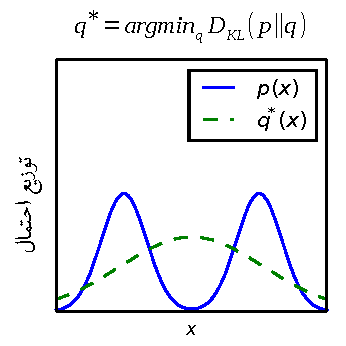
\includegraphics[scale=1]{images/KLvsReverseKL_KL.pdf}}
  			\hspace{1cm}
  			\subfigure[معکوس فاصله‌ی \lr{KL}]{\label{Figure:MLE:MLEvsReverseKL:ReverseKL}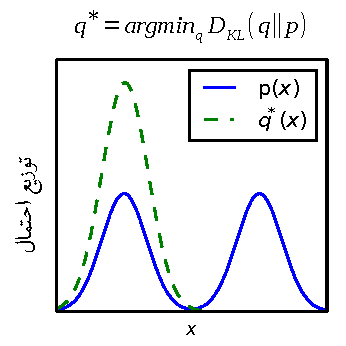
\includegraphics[scale=1]{images/KLvsReverseKL_RKL.pdf}} 
  		\end{center}
  		\caption{مقایسه رفتار بیشینه درست‌نمایی و معکوس فاصله‌ی}
  		\label{Figure:MLE:MLEvsReverseKL}
  	}
  \end{figure}
 \newline
 برای توجیه رفتار میانگین-جستجوگری، حالتی را در نظر بگیرید که این رفتار رخ ندهد یعنی محلی در فضا توزیع احتمال داده‌ی اصلی مقدار دارد و توزیع مدل به آن نقطه احتمال صفر نسبت داده است، در این شرایط تابع هزینه به سمت بی‌نهایت می‌رود و بنابر این در آموزش از چنین حالتی دوری می‌شود و هر نقطه از فضای داده که احتمال دارد، باید مدل هم احتمالی به آن نقطه نسبت دهد.
 \newline
 به عنوان یک مثالی از این رفتار، اگر فرض کنیم داده‌های واقعی توزیع دو قله‌ای گاوسی دارند و خانواده‌ی مدل مولدی که درنظر گرفته‌ایم گاوسی تک قله‌ای باشد، در شکل 
 \ref{Figure:MLE:MLEvsReverseKL:KL}
نتیجه آموزش با شرایط گفته شده نشان داده شده است، که 
 $p(x)$ 
 توزیع واقعی داده‌ها و
 $q^\star(x)$
 بهینه است. نتیجه آموزش با درست نمایی در این حالت باعث شده مدل به نقطه‌ای از فضا احتمال زیادی دهد که داده‌های اصلی احتمال کمی دارند. شکل 
 \ref{Figure:MLE:MLEvsReverseKL:ReverseKL}
 حالتی است که معکوس فاصله‌ی
 \lr{KL}
 کمینه شده و به سمتی رفته که یکی از قله‌های توزیع اصلی را یاد بگیرد که از یک جهت رفتار مناسب‌تری است. به عبارت دیگر این حالت باعث تولید نمونه‌ی نامعتبر نمی‌شود ولی می‌تواند تنوع در نمونه‌های تولیدشده را محدود کند.
\subsection{ناهماهنگی آموزش و آزمون}\label{sec1:exposurebias}
در برخی از روش‌ها نمی‌توان رفتار مشابه در آموزش و آزمون داشت که این مساله باعث می‌شود که خطایی در آموزش ایجاد شود. در ادامه به ذکر یک نمونه از این مشکل می‌پردازیم.
\newline
در اکثر روش‌ها برای تولید دنباله، مساله ساده‌سازی می‌شود و به این شکل تبدیل می‌شود که با داشتن یک زیردنباله عنصر بعدی دنباله چگونه باید باشد. 
بنابراین اگر در گام آموزش این زیردنباله‌ها فقط داده‌های واقعی باشند مشکل 
\trans{ناهماهنگی}{Inconsistency}
آموزش و آزمون پیش می‌آید، زیرا مدل فقط تصمیم گیری با دنباله‌های کاملا صحیح را آموزش دیده ولی در گام آزمون با زیردنباله‌های تولید خودش مواجه می‌شود، این مشکل اُریبی مواجهه نامیده می‌شود.
\subsection{مشکل انتقال گرادیان } \label{Problem:GradientPass}
راهکارهای زیادی برای استفاده از یادگیری مقابله‌ای در حوزه‌ی داده‌های پیوسته پیشنهاد و استفاده شده است، ولی به دلیل مشکل انتقال گرادیان در داده‌های گسسته، مستقیما امکان استفاده از این روش‌ها در حوزه‌ی داده‌های گسسته وجود ندارد.
\newline
روش بهینه‌سازیی که برای آموزش شبکه‌های عصبی استفاده می‌شود مبتنی بر محاسبه‌ی گرادیان نسبت به پارامترهای شبکه است و روش‌های یادگیری مقابله‌ای هم نیازمند محاسبه‌ی این گرادیان هستند.
برای به‌روز‌رسانی شبکه مولد لازم است که نمونه‌‌های تولید شده توسط شبکه‌ی مولد وارد دسته‌بند شده، سپس با کمک دسته‌بند تغییر پارامتر‌های شبکه‌ی مولد در جهتی که شبکه‌ی دسته‌بند فریب بخورد (یا همان گرادیان)، محاسبه ‌شود. 
برای اینکه گرادیان نسبت به پارامتر‌های شبکه‌ی مولد قابل محاسبه باشد، باید تمام عملیات ایجاد نمونه و محاسبه‌ی خروجی دسته‌بند دارای مشتق تعریف شده باشند.
\newline
در مساله‌ی تولید دنباله معمولا در انتهای شبکه‌ی مولد نیاز به نمونه‌گیری از یک توزیع است، این عملیات مشتق تعریف شده‌ای ندارد که این موضوع باعث بروز مشکل انتقال گرادیان می‌شود
\cite{SeqGAN}.
مشکل انتقال گرایان به معنی عدم توانایی انتقال گرادیان تولید شده توسط دسته‌بند به شبکه‌ی مولد است.
این چالش تنها مربوط به حوزه‌ی یادگیری مقابله‌ای نبوده و برای تقریب گرادیان پژوهش‌هایی مثل
\cite{JanGuPoo17}
انجام شده است.
در ادامه دلایل این مشکل با جزئیات بیشتر تشریح شده است.
\subsubsection{تعریف نشده بودن مشتق عملیات تصادفی}
زمانی که متغیر تصادفی $z$ تابعی از $\theta$ است و این رابطه تصادفی است، در حالت کلی مشتق $z$ نسبت به $\theta$ تعریف نشده است. این مشکل در
\trans{خود رمزگذار وردشی}{Variational Autoencoder}
هم وجود داشته و راه حل
\trans{تنظیم مجدد}{Reparametrization}
برای آن پیشنهاد شده است
\cite{JanGuPoo17}.
\newline
 برای مثال، یک نمونه استفاده از این تکنیک در رابطه با توزیع گوسی است، فرض کنید متغیر تصادفی $z$ به طوری تعریف می‌شود که
$z \sim N(f_\theta,1)$
باشد، در حالت عادی مشتق $z$ به پارامتر $\theta$ تعریف نشده است ولی با بازنویسی $z$ به صورت
$f_\theta + N(0,1)$
مشکل حل شده و با حذف قسمت تصادفی از مسیر تبدیل $\theta$ به $z$ مشتق تعریف شده است. متاسفانه در شبکه‌های مولد مقابله‌ای برای تولید دنباله، این مشکل به راحتی قابل حل نیست.
 در بخش
\ref{Method:GumbelSoftmax}
توضیحات بیشتری در این رابطه بیان شده است.
\subsubsection{گسسته بودن خروجی شبکه}
مشکل عدم وجود مشتق در مثال گاوسی به این دلیل قابل حل بوده که بعد از تکنیک تنظیم مجدد در مسیر تبدیل $\theta$ به $z$ تمام عملیات مشتق‌پذیر است.
در حالی که در تولید دنباله گسستگی مقادیر، تعریف دقیق مشتق را ناممکن می‌کند و تنها راه‌کارهای تقریبی ممکن هستند. شبکه‌ا‌ی که در مساله‌ی تولید دنباله گسسته استفاده می‌شود نیازمند تولید داده‌های گسسته است و بنابراین خروجی شبکه‌ی مولد نوع گسسته دارد.
\newline
مشکل گسسته بودن خروجی عملیات را از دو دیدگاه می‌توان بیان کرد.
دیدگاه اول اینکه برای مشتق این عملیات راه حلی نداریم و راه عملی برای انجام آن وجود ندارد. برای مثال در نظر بگیرید رابطه‌ی 
${z = \argmax_i f_i(\theta)}$
برای $z$ برقرار است و می‌خواهیم مشتق $z$ نسبت به $\theta$ را محاسبه کنیم که روش برای آن نداریم.
دیدگاه دوم به صورت بررسی هندسی است، فرض کنید تابع $f$ به صورت 
${z=f(\theta)}$
تعریف شده است و خروجی آن گسسته است، یعنی $z$ دارای $N$ حالت ممکن است. فضایی که پارامتر‌های 
$\theta$
می‌سازند را در نظر بگیرید، از آنجا که در کل $N$ حالت خروجی وجود دارد، بنابراین فضای پارامتر‌های $\theta$ به $N$ بخش افراز می‌شود. اگر $\theta$ نقطه‌ای در یکی از نواحی فضا باشد با تغییرات محلی در مقدار $\theta$ خروجی تغییری نمی‌کند و مشتق معنی ندارد
\cite{SeqGAN}
، شکل 
\ref{Figure:DiscreteSpace}
توصیفی از چنین فضایی است.
\begin{figure}[!htb]
	\centering
	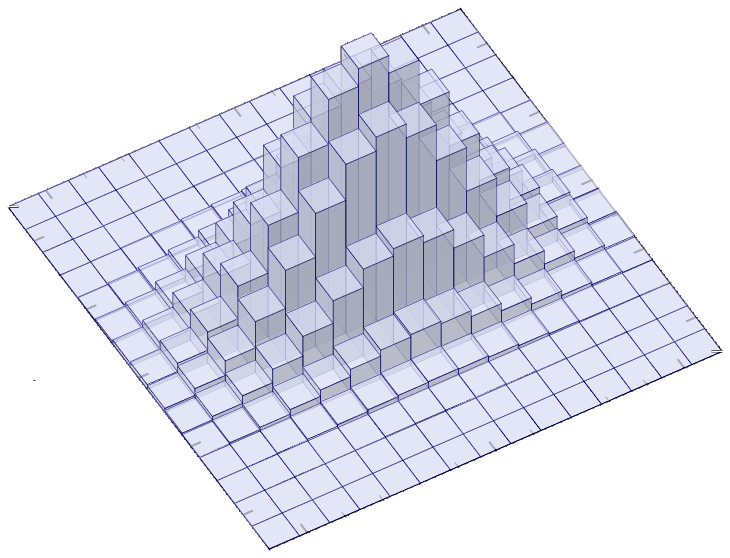
\includegraphics[width=0.5\textwidth]{images/DiscreteSpace.png} 
	\caption[ نمایش یک نمونه تابع از مقدار پیوسته‌ی دو بعدی به یک مقدار گسسته]
	{
		نمایش یک نمونه تابع از مقدار پیوسته‌ی دو بعدی به یک مقدار گسسته، در چنین فضایی روش‌های مبتنی بر گرادیان برای پیدا کردن نقطه‌ی بیشینه کارساز نیست.
	}
	\label{Figure:DiscreteSpace}
\end{figure}
\subsection{ناپایداری آموزش مقابله‌ای} \label{Problem:GANinstablity}
 	\begin{figure}[!htb]
 		{
 			\begin{center}
 				\subfigure[آموزش ناپایدار]{\label{Figure:GANInstability:Bad}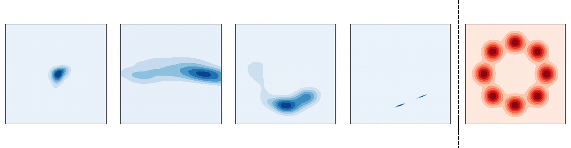
\includegraphics[scale=1.1]{images/GANBadTrain.pdf}}
 				\hspace{1cm}
 				\subfigure[آموزش پایدار]{\label{Figure:GANInstability:Good}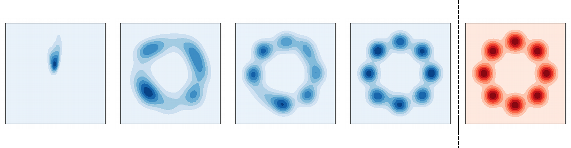
\includegraphics[scale=1.1]{images/GANGoodTrain.pdf}} 
 				\end{center}
 			\caption[نمایش ناپایداری آموزش شبکه‌های مولد مقابله‌ای و پایدارکردن آن ]{
 				نمایش ناپایداری آموزش شبکه‌های مولد مقابله‌ای و پایدارکردن آن با روش معرفی شده در
 				\cite{Mescheder17TheNumericOfGan}.
 				تصویر سمت راست توزیع داده‌ی اصلی را نشان می‌دهد و بقیه تصاویر از چپ به راست توزیع مدل مولد در حین آموزش و در گام‌های ۰، ۵۰۰۰، ۱۰۰۰۰ و ۲۰۰۰۰ آموزش است.
 			}
 			\label{Figure:GANInstability:BadAndGood}
 		}
 		\end{figure}
بزرگترین چالشی که در روش‌های آموزش مقابله‌ای وجود دارد ناپایداری آموزش آن است.
دو نمونه‌ از این ناپایداری به شرح زیر است:
\begin{itemize}
	\item 
آموزش مقابله‌ای می‌تواند به رفتار ناپایداری منجر شود که توزیع مدل مولد بین چند قله از توزیع اصلی به صورت تناوبی جابجا شود که این رفتار
 \trans{چسبیدگی به قله}{Mode Collapsing}
 نام دارد.
 یک مثال از چسبیدگی به قله در شکل
 \ref{Figure:GANInstability:Bad}
 نشان داده شده است و نشان می‌دهد که در آموزش یک توزیع چندقله‌ای به عنوان توزیع اصلی، مدل مولد بین قله‌ها به صورت تناوبی جابجا می‌شود.
 هم‌چنین شکل
 \ref{Figure:GANInstability:Good}
 نشان دهنده‌ی حالتی است که با تکنیک معرفی شده در
 \cite{Mescheder17TheNumericOfGan}،
 این آموزش پایدار شده است.
 \item
 مشکل دیگر در تکنیک مطرح‌شده در تنظیم نسبت آموزش مدل‌ مولد و تمیزدهنده است. به این صورت که اگر مدل تمیزدهنده به خوبی آموزش ببیند تمام نمونه‌های مدل مولد را به راحتی تشخیص می‌دهد و این موضوع باعث سخت شدن آموزش مولد می‌شود. مثلا فرض کنید شبکه‌ی مولد بر اساس امتیازی که از تمیزدهنده می‌گیرد آموزش می‌بیند و در حالتی که تمیزدهنده خیلی قویتر باشد به همه‌ی حرکت‌های خوب مولد امتیاز بسیار کوچکی می‌دهد که این موضوع باعث آموزش ندیدن مولد در عمل می‌شود. در واقع نزدیک نقطه‌ی بهینه برای تمیزدهنده، گرادیان نزدیک صفر است و چندان نمی‌تواند به بهبود مولد کمک کند.
\end{itemize}
 برای پایدار کردن آموزش روش‌هایی ارائه شده است
 \cite{Arjovsky17Wasserstein, Gulrajaniy17ImprovedWasserstein, Mescheder17TheNumericOfGan, Roth18StabilizeGAN, Luke16UnrolledGAN,Salimans16ImprovedTechTrainingGAN}،
 ولی بسیاری از این روش‌ها خاص حوزه‌ی داده‌های پیوسته است و نمی‌توان از آنها در تولید دنباله مستقیما بهره برد.
\section{هدف پژوهش}
با توجه به تعریف مساله در بخش 
\ref{sec:chap1:definition}
و چالش‌هایی که برای حل آن وجود دارد، در ادامه قصد داریم روشی برای تولید دنباله ارائه کنیم که بر پایه‌ی شبکه‌های مولد مقابله‌ای است، اما با مشکلاتی نظیر انتقال گرادیان رو به رو نیست. هم‌چنین در جهت ارزیابی موثرتر مدل پیشنهادی، معیارهای سنجش کیفیت را مورد مطالعه‌ی دقیق قرار داده و معیارهای جدیدی را برای این منظور پیشنهاد می‌کنیم.

\section{ساختار پایان‌نامه}
در ادامه‌ی مستند حاضر، در فصل دوم به تشریح کار‌های پیشین در زمینه‌ی تولید دنباله می‌پردازیم و با بررسی مزایا و معایب این روش‌ها، رویکردهای مختلف حل این مساله را با یکدیگر مقایسه می‌کنیم و در فصل سوم راهکار پیشنهادی برای تولید دنباله را معرفی می‌کنیم.
از آنجا که معیار ارزیابی خود موضع چالش برانگیزی در این حوزه است فصل چهار را به تشریح این معیارها می‌پردازیم و معیارهای جدیدی را پیشنهاد می‌کنیم. با ارائه آزمایش‌های انجام شده در فصل پنجم، به ارزیابی روش پیشنهادی می‌پردازیم. در نهایت با جمع‌بندی مطالب ارائه شده و ارائه پیشنهاداتی برای ادامه پژوهش، پایان‌نامه را به پایان می‌بریم.



